%File: submission_revised.tex --- AAAI-27 anonymous submission
% "An Empirical Analysis of Transfer for Dynamic Path Planning"
% Built on the official AAAI-27 author kit (aaai2027.sty, TemplateVersion 2027.1).
\documentclass[letterpaper]{article} % DO NOT CHANGE THIS
\usepackage[submission]{aaai2027}  % DO NOT CHANGE THIS
\usepackage[hyphens]{url}  % DO NOT CHANGE THIS
\usepackage{graphicx} % DO NOT CHANGE THIS
\urlstyle{rm} % DO NOT CHANGE THIS
\def\UrlFont{\rm}  % DO NOT CHANGE THIS
\usepackage{natbib}  % DO NOT CHANGE THIS AND DO NOT ADD ANY OPTIONS TO IT
\usepackage{caption} % DO NOT CHANGE THIS AND DO NOT ADD ANY OPTIONS TO IT
\frenchspacing  % DO NOT CHANGE THIS
%
% Recommended for better-looking tables
\usepackage{booktabs}
\usepackage{amsmath}
%
\pdfinfo{
/TemplateVersion (2027.1)
}
\setcounter{secnumdepth}{0}

% Custom macros
\newcommand{\stage}[1]{\textsc{#1}}

\title{An Empirical Analysis of Transfer for Dynamic Path Planning}
\author{
    Anonymous Submission
}
\affiliations{
}

\begin{document}

\maketitle

\begin{abstract}
We study the dynamic path planning problem, where an agent needs to plan a route in the presence of moving obstacles. This problem is relevant for all agents that need to navigate in the real world. In particular, we study whether heuristics learned in training maps can be transferred---zero-shot or from a few labeled target maps---to new environments for this task. We show that, with the right training objective and planner integration, heuristics transfer zero-shot in both discrete and continuous environments---even heuristics given no information about future obstacle motion---matching or improving success in new maps while substantially reducing search effort. With a few labeled target maps, low-rank adaptation preserves the transferred prior while full fine-tuning overtakes it as labels accumulate---and a single dynamic map is already label-rich. Further, this is agnostic to model architecture choices in that Multilayer Perceptrons, Long Short-Term Memory models, Hierarchical Reasoning Models and U-Net architectures of comparable complexity all can be used with similar success rates.
\end{abstract}

% Uncomment the following to link to an anonymous code/data archive included with the submission.
% Keep this block between (not within) the abstract and the main body.
% \begin{links}
%     \link{Code and Data}{https://anonymous.example/}
% \end{links}

\section{Introduction}

An agent navigating the real world rarely plans on an empty, static map: pedestrians cross corridors, vehicles occupy lanes, and doors open and close. Planning in the presence of moving obstacles---the \emph{dynamic path planning} problem---is harder than static path planning because search must reason over space and time \citep{silver2005cooperative,phillips2011sipp}. The simple admissible heuristics that make A\textsuperscript{*} \citep{hart1968astar} efficient on static maps become weak once waiting, detouring, and timing matter. Learned heuristics can reduce search effort \citep{arfaee2011bootstrap,bhardwaj2017sail,yonetani2021neuralastar}, but a deployed agent benefits only if a heuristic trained on one set of maps remains useful on maps it has never seen. We therefore ask: \emph{when do learned heuristics transfer zero-shot, or after adaptation from a few labeled target maps, to new environments for dynamic path planning?}

A fair answer requires separating transfer from three confounds: the target representation used to train the heuristic, the way the prediction enters the planner, and the amount of supervision contained in one ``shot.'' We use static suites as a controlled proving ground, then test the resulting claims under deterministic dynamics. The program pairs interventions with matched controls: twin models differing in one input, identical frozen weights under different planner integrations, calibrated budgets at which the classical baseline is neither saturated nor hopeless, and map-level paired inference for repeated evaluations \citep{henderson2018matters,agarwal2021precipice,pineau2021reproducibility}. Across thirteen stages---with written designs, gates, budgets, and analysis grains frozen before execution from \stage{C7} onward---our central finding is that \emph{transfer depends more on representation, planner integration, and supervision density than on nominal model hierarchy}.

Our contributions are:
\begin{itemize}
    \item \textbf{Calibrated evidence for zero-shot transfer.} On six continuous static suites, selected transferred providers reduce matched expansions by 15--48\%, with corrected success evidence on four suites. On six dynamic suites, selected providers reduce matched expansions by 62--95\% and improve success on five suites, subject to small matched sets in two cells. A smaller discrete pilot finds 6--15\% reductions in the tested cells when the same frozen model is used as a focal ranker.
    \item \textbf{A cross-domain integration result.} Changing the target representation rescues a collapsed recurrent backbone; changing only the planner integration turns an inert discrete residual into useful guidance; and sharing search state turns an exact oracle from a six-map loss into a six-map win. These controls show that apparent transfer or architecture failures can be harness failures.
    \item \textbf{A supervision-density account of adaptation.} With scarce static labels, rank-8 LoRA preserves the transferred prior while full fine-tuning is unstable; with more labels, full fine-tuning often overtakes it. Bounded and unbounded LoRA are nearly identical, implicating low-rank capacity rather than the output clamp. One dynamic map already supplies roughly 25{,}000 space--time labels, so the static crossover leaves its low-data regime.
    \item \textbf{Controlled negative and constructive mechanism results.} Future-window inputs, descriptor-weighted adapter interpolation, and hierarchical depth provide no consistent benefit under the tested formulations. As a constructive stress test under restricted information, a small local-observation MLP plus one inference-time Bellman backup reduces expansions by 15.95\% against a frozen complete-map comparator on 144 held-out static maps, with explicit path-quality, safety, and runtime qualifications.
\end{itemize}

Figure~\ref{fig:map} organizes the program by the causal question each stage addresses. Table~\ref{tab:matrix} gives the evidence-safe conclusions and their scope.

\begin{table*}[t]
\centering
\footnotesize
\begin{tabular}{@{}p{2.3cm}p{2.0cm}p{7.3cm}p{4.2cm}@{}}
\toprule
Question & Stages & Evidence-safe conclusion & Main qualification \\
\midrule
Representation and integration & \stage{C5--C8}; discrete; \stage{C13-C--D} & Target structure and planner coupling can reverse the result without establishing an architecture or transfer failure: scalar collapse is repaired by field training; additive and focal integration invert across loose and tight baselines; shared search state rescues an exact oracle. & Continuous headlines are mostly local, one-primary-seed validations; the discrete focal result is a limited 3--8-seed pilot. \\
Adaptation and composition & \stage{C9/C9h};\newline\stage{C9b/C10} & LoRA preserves a strong prior in the static low-label regime; full fine-tuning exploits larger label sets; one dynamic map is already label-rich. Descriptor-weighted composition does not consistently beat the pooled zero-shot provider. & Direct equivalence is not claimed; repeated adaptation seeds are aggregated within test maps for inference. \\
Architecture and depth & \stage{C11/C12}; \stage{C13-N/O/P} & No stable hierarchy-specific or depth dose--response appears. Global-input models separate at shallow missions, recurrent collapse affects several cells, iterative cycles help search but not preferentially at greater depth, and persistent carry loses to a reset twin. & These are formulation-specific negatives, not claims that recurrence, memory, or hierarchy are universally useless. \\
Restricted-information transfer & \stage{C13-A--M} & After target, distribution, and static-integration repairs fail, one bounded local Bellman backup produces a frozen 144-map confirmation win over complete-map providers. & Static stress test; one model seed and cohort; direct arm is not formally bounded and is slower in wall time. \\
\bottomrule
\end{tabular}
\caption{The experimental program grouped by claim rather than chronology. Full per-suite tables, protocols, and statistical details are in the technical appendix.}
\label{tab:matrix}
\end{table*}

\begin{figure*}[t]
\centering

\includegraphics[width=0.98\textwidth]{figures/fig1_program_map.pdf}
\caption{The program as a sequence of controlled questions. Representation studies test whether the target exposes usable structure; integration studies test whether identical predictions can affect search; adaptation studies vary supervision density; architecture studies test hierarchy only after establishing task headroom. Orange denotes a failed or negative gate, blue a positive result under the corrected harness, and gray a mechanism or diagnostic result.}
\label{fig:map}
\end{figure*}

\section{Experimental Setting and Evaluation}

\textbf{Planning tasks.} The discrete program uses receding-horizon space--time A\textsuperscript{*} on grids with Manhattan distance as the classical heuristic. The continuous program uses a 2-D point robot and a probabilistic roadmap \citep[PRM;][]{kavraki1996prm} of approximately 192 nodes with $k{=}7$ connectivity; Euclidean distance is the classical heuristic. In dynamic suites, the search state is $(\text{node},t)$ and obstacles follow deterministic trajectories. Each suite has a binding node-expansion budget calibrated so that the classical baseline is neither saturated nor hopeless. Success means reaching the goal within that budget.

\textbf{Labels and providers.} Static continuous labels are exact graph-Dijkstra costs-to-go; dynamic labels are exact backward space--time Dijkstra values. The program studies scalar residual regressors and goal-conditioned raster residual fields sampled at PRM nodes. Backbones include MLPs, LSTMs \citep{hochreiter1997lstm}, ON-LSTMs \citep{shen2019onlstm}, Hierarchical Reasoning Models \citep[HRMs;][]{wang2025hrm} including an adaptive-computation port \citep{graves2016act,banino2021pondernet}, FiLM-conditioned U-Nets \citep{ronneberger2015unet,perez2018film}, and graph networks. Arms are parameter-matched where the experiment makes a direct architecture comparison; the paper does not treat parameter counts from unrelated stages as a global match.

\textbf{Transfer protocol.} We distinguish unseen maps from trained families, unseen map families, and a final restricted-observation setting. Zero-shot transfer applies a frozen provider. Few-shot adaptation uses $K$ labeled target maps and compares rank-8 LoRA \citep{hu2021lora}, full fine-tuning, and training from scratch. In the later compositional study, $K$ instead denotes mission length; we state that use explicitly to avoid conflating the two quantities.

\textbf{Metrics and inference.} We report success and matched-solved expansion ratios separately. The ratio is learned-arm expansions divided by baseline expansions on maps both solve; it conditions on joint success and can favor an arm that solves only easier maps. Success is compared with paired McNemar tests and Benjamini--Hochberg correction within stage families. Expansion ratios use percentile bootstrap intervals, and path-cost ratios are reported separately. For stages that repeat adaptation or model seeds on fixed test maps, seeds are averaged within maps before inference; quoted \stage{C9--C11} contrasts use map-clustered bootstraps or stratified permutation. Most continuous headline stages use one primary training seed unless stated; \stage{C11} and \stage{C12} include multi-seed grids. From \stage{C7} onward, designs and analysis grains were frozen before execution, and confirmation cohorts were generated only after model and integration choices were fixed.

\section{Harness Effects: Representation and Integration}

The proviso in the abstract---\emph{with the right training objective and planner integration}---is an empirical result, not a generic caveat. Both choices can create an apparent transfer or architecture failure even when the learned signal is useful.

\textbf{Target representation.} On calibrated hard static maps (\stage{C5}), a pooled ON-LSTM scalar residual regressor raises hard-maze success from 0.525 to 1.000 over Euclidean A\textsuperscript{*} (corrected $q=4.3\times10^{-11}$), while the HRM scalar arm collapses to a constant at the normalization cap and matches the baseline. Lower learning rates and a soft-cap follow-up reproduce the collapse. \stage{C6} retains an HRM backbone but changes the target/output structure to a goal-conditioned raster residual field; hard-maze success rises from 0.625 to 0.975 ($q=3.4\times10^{-4}$). \stage{C7} then shows that a well-trained scalar HRM can also work (per-suite ratios 0.427--0.822). The evidence therefore localizes the earlier failure to the target/optimization path; it does not establish that value fields are intrinsically necessary or that HRM is intrinsically unsuitable.

\begin{figure}[t]
\centering

\includegraphics[width=0.98\columnwidth]{figures/fig2_integration.pdf}
\caption{The integration inversion. Against a tight Manhattan baseline on discrete grids, additive learned magnitude is inert or harmful, whereas the same frozen predictions reduce expansions by 6--15\% as a ranker inside the tested focal band. Against a loose Euclidean baseline on continuous hard roadmaps, additive guidance reduces matched expansions by 15--48\%; focal variants recover less.}
\label{fig:integration}
\end{figure}

\textbf{Planner integration.} The useful interface depends on baseline tightness (Figure~\ref{fig:integration}). On continuous hard roadmaps, additive learned heuristics exploit the gap left by Euclidean distance: the field-HRM ratios in \stage{C7} are 0.521--0.850, with empirical path-cost ratios approximately 1.02--1.14, while focal variants are closer to Euclidean search. On discrete grids, the pooled residual has correlation 0.987--0.994 with the true residual across tested map sizes, but its magnitude is scale-flat: the predicted-to-true mean falls from 0.73 to 0.19 as maps grow. Added to tight Manhattan distance, every learned arm in the controlled 22-suite run is at or below the matched baseline. Reusing the same frozen predictions only to rank states within a focal band at $w=1.0$ reduces expansions by 6--15\% in the tested cells without an observed success regression, supporting rank-oriented heuristic learning \citep{chrestien2023rank}.

A later oracle control isolates integration more directly. An exact value ranker combined with a fresh, work-discarding certifier loses all six primary comparisons (141.2 versus 129.7 expansions). Sharing one search state changes no oracle values, yet wins all six (122.8 expansions). The lesson is narrower than a universal recipe: objective and integration must be validated before a transfer or architecture verdict is interpretable.

\section{Zero-Shot Transfer}

\textbf{Static maps and held-out families.} On six calibrated static PRM suites---three training families and three held out---the transferred field HRM solves 0.75--1.00 of test maps against Euclidean success of 0.25--0.58. Corrected success evidence holds on four suites, and matched expansion ratios are 0.521--0.850 (\stage{C7}). Family-level transfer is also visible in \stage{C9}: frozen pooled providers improve success over Euclidean A\textsuperscript{*} in all six target/backbone cells ($q<0.001$--$0.025$), before any target labels are used.

\textbf{Dynamic maps.} \stage{C8} uses six suites with deterministic moving obstacles and exact space--time labels. The selected strongest learned arm in each suite raises success from 0.05--0.75 to 0.75--1.00 and has matched expansion ratios 0.046--0.380. Corrected success evidence holds on five suites; rooms-large is supported mainly by expansion evidence. Two ratios require particular care: dense maze has only one jointly solved map at the binding budget and therefore supports no expansion inference, and spiral has four. The defensible headline is thus that selected transferred providers substantially improve search in these local dynamic benchmarks, not that every architecture or suite has a precisely estimated 62--95\% reduction.

\textbf{Future-window inputs provide no consistent benefit.} The dynamic study trains aware/blind twins that differ only in an eight-step future-obstacle window. Across 24 suite-by-backbone cells, one uncorrected significant comparison favors the aware twin and seven favor the blind twin; direct heuristic MAE favors aware in 11 cells and blind in 13. After full fine-tuning on $K=16$ target maps, eight of nine map-level success point differences are non-positive and the sole positive interval still includes zero. We therefore report a failure to observe a systematic future-window benefit, not equivalence or harm. Future prediction was not necessary for the gains on these deterministic suites; stochastic motion remains untested.

\textbf{Discrete transfer.} In the complete pooled-multitask run, the HRM average base improves mean success from 0.591 to 0.612 and lowers mean expansions (descriptive); task-specific adapters do not improve broadly. The focal result is smaller in scope: a local 3--8-seed pilot on selected 128- and 192-cell maps finds 6--15\% expansion reductions at $w=1.0$ with equal or higher observed success. It is evidence that transferable ordering survived scale shift, but not yet a full-suite confirmation.

\begin{figure*}[t]
\centering
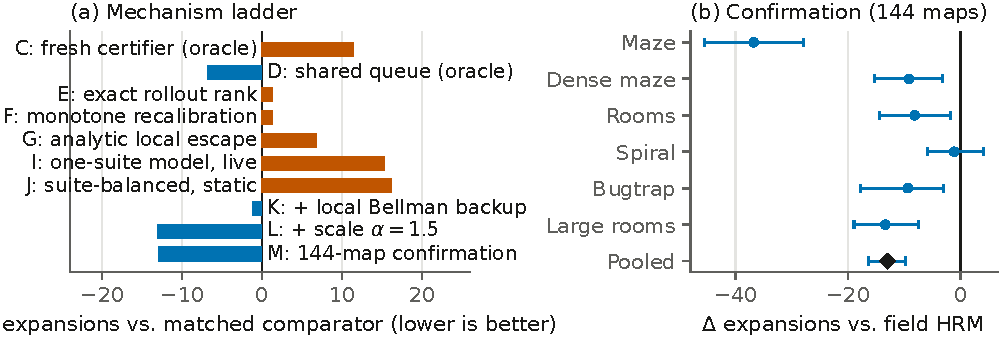
\includegraphics[width=0.98\textwidth]{figures/fig5_c13.pdf}
\caption{Restricted-observation stress test (\stage{C13}, static). (a) Each rung changes one factor. Exact behavior returns, analytic local targets, one-family training, and suite-balanced static insertion fail; one radius-bounded Bellman backup at inference changes the sign. (b) After freezing the iteration, backup, and scale, a disjoint 144-map cohort yields a pooled expansion delta of $-12.96$ (95\% CI $[-16.30,-9.74]$; 109/3/32 wins/ties/losses) against the preregistered complete-map field-HRM comparator, with every suite mean negative and better empirical path-cost ratios.}
\label{fig:ladder}
\end{figure*}

\textbf{Restricted-observation stress test (static).} The final study asks whether the mechanism survives when the learned provider cannot condition on complete-map features at query time. The planner still knows the PRM, but the provider sees only a radius-0.20 local subgraph and is trained from fresh-start behavior returns rather than shortest-path labels. This is a static mechanism study, not additional evidence about moving obstacles.

The falsification ladder in Figure~\ref{fig:ladder}a separates target, representation, distribution, and integration. The exact behavior-return statistic itself loses to matched focal search; two analytic local-escape targets are too weak; a one-family model loses across the six-suite distribution by $+15.36$ expansions (95\% CI $[+12.02,+18.64]$); and suite-balanced training still loses by $+16.17$ under static insertion. Adding one radius-bounded Bellman backup at inference changes the same checkpoint's development delta to $-1.21$; scale calibration on fresh maps reaches $-13.04$ (CI $[-18.67,-7.65]$).

After freezing the model, integration, and analysis, a disjoint 144-map cohort (24 per family) yields 68.31 expansions for the restricted-observation MLP versus 81.26 for the preregistered complete-map field HRM: paired delta $-12.96$, 95\% CI $[-16.30,-9.74]$, 109/3/32 wins/ties/losses, and a negative mean in every suite (Table~\ref{tab:c13m}). The frozen provider table also places the local MLP below every fixed \stage{C7} learned provider in pooled expansions. Empirical mean/max cost ratios improve from 1.031/1.335 to 1.024/1.162. A separate $w=1.10$ control passes every bound and certificate check. The direct arm itself is not formally bounded, uses one model seed and one cohort, and has a slower prototype feature builder; this is a search-effort/path-quality result rather than a wall-clock claim.

\begin{table}[t]
\centering
\small
\begin{tabular}{lcc}
\toprule
 & Local MLP & Field HRM \\
\midrule
Mean expansions $\downarrow$ & \textbf{68.31} & 81.26 \\
Paired $\Delta$ [95\% CI] & \multicolumn{2}{c}{$-12.96$ $[-16.30,-9.74]$} \\
Win / tie / loss & \multicolumn{2}{c}{109 / 3 / 32} \\
Negative suite means & \multicolumn{2}{c}{6 / 6} \\
Mean cost ratio $\downarrow$ & \textbf{1.0235} & 1.0311 \\
Max cost ratio $\downarrow$ & \textbf{1.1624} & 1.3346 \\
Valid paths & 144 / 144 & 144 / 144 \\
Feature build (s/map) $\downarrow$ & 5.138 & \textbf{0.371} \\
\bottomrule
\end{tabular}
\caption{Frozen \stage{C13-M} confirmation on 144 untouched static maps (one model seed). Cost ratios are relative to graph-optimal cost. A separate bounded control passes all 144 safety checks.}
\label{tab:c13m}
\end{table}

\section{Few-Shot Adaptation}

\begin{figure}[t]
\centering
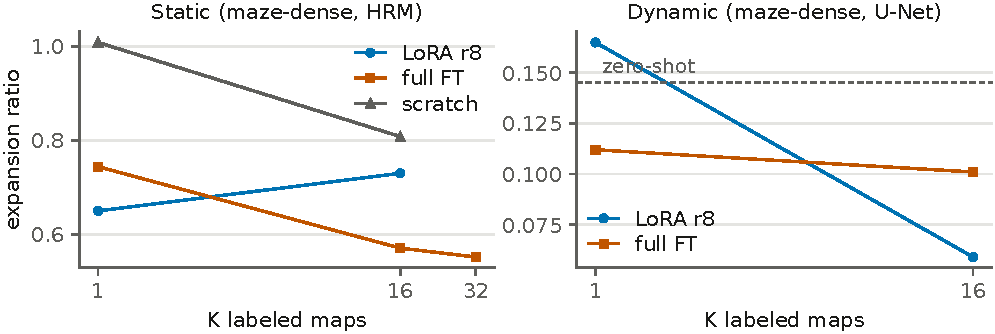
\includegraphics[width=0.98\columnwidth]{figures/fig3_transfer.pdf}
\caption{Supervision density organizes few-shot adaptation. Left: on static targets, rank-8 LoRA preserves the prior at $K=1$, while full fine-tuning can fail early and often wins by $K=8$--16. Right: one dynamic map provides roughly 25{,}000 $(\text{node},t)$ labels, and the low-label crossover disappears. Points show the canonical curves; quoted inference in the text is map-clustered.}
\label{fig:transfer}
\end{figure}

Adaptation behavior is better indexed by labeled states than by labeled maps.

\textbf{Scarce static labels preserve the prior.} At $K=1$, maze-dense HRM LoRA has a map-level ratio of 0.686 (95\% CI $[0.590,0.774]$) and a success delta of $+0.467$ ($[+0.300,+0.633]$). Full fine-tuning is unstable in this regime: on rooms-large, its $K=1$ ratio is 1.293 ($[1.170,1.503]$), while scratch on maze-dense has success delta $-0.167$ ($[-0.300,-0.047]$) and ratio 1.035. These cells show what transfer contributes at low data: a useful prior that adaptation can preserve or destroy.

\textbf{More labels expose full-rank capacity.} By $K=8$--16, full fine-tuning often overtakes LoRA. On maze-dense at $K=16$, the map-level intervals are disjoint: 0.610 $[0.549,0.670]$ for full fine-tuning versus 0.786 $[0.694,0.891]$ for LoRA. A matched-compute ablation isolates the LoRA plateau: across 27 cells, bounded-minus-unbounded map-level ratio differences have median 0.0000, standard deviation 0.0077, and maximum absolute difference 0.037. This is strong descriptive evidence for a rank-capacity bottleneck, not a formal equivalence test. LoRA is also not universally base-preserving: bugtrap degrades significantly by $K=32$ (ratio 1.153, CI $[1.012,1.523]$).

\textbf{Dynamic maps are label-rich.} One dynamic map yields approximately $192$ nodes times about $140$ time steps, or more than 25{,}000 supervised states. Full fine-tuning is therefore no longer systematically catastrophic at $K=1$, and LoRA can continue to improve rather than merely preserve the base. Scratch arms can show attractive solved-only ratios while solving fewer maps, so success must lead those comparisons. The result is a regime shift in supervision density, not a universal law about the number of maps.

\textbf{Composition does not improve the prior.} A zero-label alternative interpolates 16 family experts using target descriptors. Routing identifies the correct family axis (own-axis mass 0.986--0.998), yet map-paired composition never improves significantly over the pooled zero-shot provider and is significantly worse in two of six cells (up to $+0.098$ expansions-ratio delta, CI $[+0.076,+0.123]$). Weight-space and prediction-space mixtures are nearly identical. This negative result complements work on model averaging and task arithmetic \citep{wortsman2022soups,ilharco2022task}: accurate routing is insufficient when experts have not moved beyond a strong pooled base.

\section{What Architecture Explains}

\begin{figure}[t]
\centering
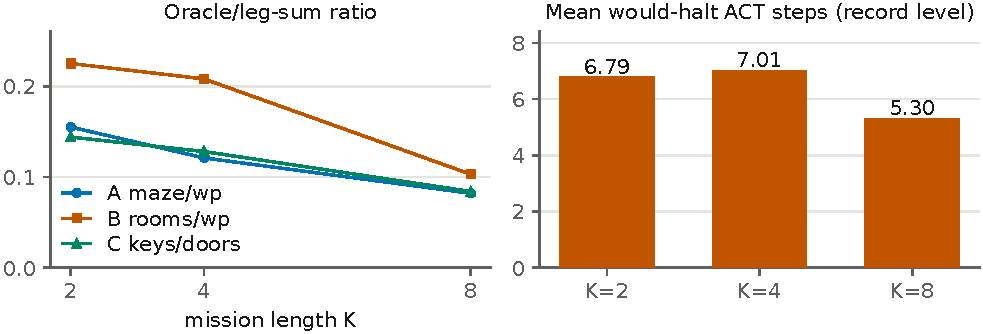
\includegraphics[width=0.98\columnwidth]{figures/fig4_c11.pdf}
\caption{Testing hierarchy with compositional headroom (\stage{C11}). Here $K$ denotes mission length, not adaptation maps. The exact oracle's ratio over a leg-sum baseline falls as missions deepen, but learned HRM halting uses fewer steps at $K=8$; the map-level anti-correlation is $\rho=-0.578$ ($p=5\times10^{-5}$).}
\label{fig:c11}
\end{figure}

Across the transfer studies, no architecture has a stable advantage across tasks. This is narrower than saying architecture is irrelevant. U-Net is often strongest in the dynamic field study, HRM has the lowest single-suite dynamic ratio, ON-LSTM is strongest in the early calibrated scalar stage, and the ordering reverses on separate forecasting tasks. Architecture comparisons are therefore conditional on information access, target representation, optimization, and planner integration.

\textbf{No hierarchy-specific depth response.} \stage{C11} deliberately creates compositional multi-leg missions with enough oracle headroom for a depth-sensitive method to improve. Here $K\in\{2,4,8\}$ is mission length. The main grid contains six learned arms, three seeds, 198 checkpoints, and 54{,}450 evaluation rows. No structured arm beats the MLP at two depths with a non-decreasing gap; forced HRM-v2 compute produces nearly flat error and expansion curves; and learned halting moves opposite to the hypothesis. Mean would-halt steps are 6.79/7.01/5.30 at $K=2/4/8$, with map-level $\rho=-0.578$ and stratified permutation $p=5\times10^{-5}$ (Figure~\ref{fig:c11}).

The experiment does reveal an information-structure effect: U-Net/GNN arms with global inputs separate from the MLP at shallow $K$ in two configurations, with ratios approximately 0.67--0.87, but every $K\in\{4,8\}$ interval includes parity. Five of 33 recurrent/ACT arm-cells exhibit full or partial constant-prediction collapse; their worst deep-mission rows are optimization-pathology measurements, not clean capacity estimates. A 12-run scaled U-Net/HRM follow-up preserves the ordering and the deep HRM collapse.

\textbf{Two rescue hypotheses remain negative.} \stage{C12-A} constructs hidden slow/fast regimes with substantial memory-relevant headroom, yet the frozen one-seed learned pilot fails forecast, planning, and persistent-carry gates. \stage{C12-B} gives a product-graph refiner up to eight recurrent cycles. Search burden improves monotonically with cycles in all four cells, but the gain is no larger at $K=8$ than at $K=2$; a tied-control win on one configuration reverses on another, and Bellman residual worsens with cycles. Recurrent compute can improve bounded search without supporting the proposed hierarchy/depth mechanism \citep{tamar2016vin,lee2018gppn}.

\textbf{Substitution and persistent state do not recover the local result.} Replacing the confirmed local MLP with a trimmed HRM improves pooled expansions relative to field HRM on the development block, but fails suite-robustness and matched-MLP path-quality gates; changing the readout order helps transiently and fails at the frozen endpoint. A same-checkpoint persistent-versus-reset pilot then gives the recurrent model state across the entire query. Persistent carry worsens world-macro frontier ranking (MRR delta $-0.0294$, 95\% CI $[-0.0598,-0.0030]$), and no confirmation is opened. Recent simplification results for recursive reasoning models \citep{jolicoeur2025trm} provide related motivation, but operate on different benchmarks. Our conclusion is limited to the tested heuristic formulations: we find no robust benefit attributable specifically to hierarchy, while planner-side hierarchy such as learned subgoals remains outside scope \citep{czechowski2021subgoal}.

\section{Related Work}

\textbf{Learned guidance for search.} Learned heuristics have been trained by bootstrapping \citep{arfaee2011bootstrap}, oracle imitation \citep{bhardwaj2017sail}, differentiable search \citep{yonetani2021neuralastar}, transformer-based grid guidance \citep{kirilenko2023transpath}, and supervised classical-planning objectives \citep{ferber2020neural}. We complement this literature by isolating cross-map transfer from target, integration, and supervision-density effects. The discrete focal result is especially close to ranking-oriented objectives \citep{chrestien2023rank}. Bounded-suboptimal and multi-heuristic search provide alternative interfaces for learned signals \citep{pohl1970,pearl1982semiadmissible,aine2016mha}.

\textbf{Dynamic, real-time, and motion planning.} The dynamic substrate follows space--time and safe-interval search \citep{silver2005cooperative,phillips2011sipp}. The restricted-observation study is related to real-time heuristic search \citep{korf1990rta} and local value updates in Real-Time Adaptive A\textsuperscript{*} \citep{koenig2006rtaa}; its one-step backup also resembles a single value-iteration-network update \citep{tamar2016vin,lee2018gppn} and neural algorithm execution more broadly \citep{velickovic2021nar}. Learned samplers and end-to-end motion planners \citep{ichter2018sampling,qureshi2019mpnet} are complementary: we retain a classical planner and learn only its guidance, making frozen transfer measurable on a PRM \citep{kavraki1996prm}.

\textbf{Adaptation and recursive architectures.} LoRA \citep{hu2021lora}, model soups \citep{wortsman2022soups}, and task arithmetic \citep{ilharco2022task} motivate the low-rank and composition studies. HRM \citep{wang2025hrm}, adaptive computation \citep{graves2016act,banino2021pondernet}, and simplified recursive models \citep{jolicoeur2025trm} motivate the hierarchy audit. Our results concern heuristic regression and planner integration rather than the benchmark claims of those architectures.

\section{Limitations}

Most continuous headline results are local single-GPU validations with one primary training seed, and several stages reuse bases or test maps rather than constituting independent replications. The strongest dynamic ratios come from selected arms; dense maze has one jointly solved map at its binding budget, and the spiral cell has four. The discrete focal result covers selected cells with 3--8 seeds, not the full 22-suite matrix. Map-clustered reanalysis supports the quoted \stage{C9--C11} verdicts, but not every exploratory full-grid table has been regenerated at that grain, and no equivalence tests were run.

The \stage{C13-M} confirmation is static, uses one model seed and one 144-map cohort, and should be read as a mechanism stress test rather than direct evidence about moving obstacles. Its provider is locally restricted but the planner still knows the PRM; this is not map-free sensing. The direct operating point has no formal suboptimality bound, while the certified control is slower. The prototype local-feature builder also makes the method slower in wall time than complete-map field inference despite fewer expansions.

Dynamic obstacles are deterministic, and the work does not cover stochastic prediction, kinodynamic constraints, multi-agent coupling, physical robots, or environments beyond 2-D single-agent navigation. Negative results are failures to observe improvement under the frozen protocols, not universal rejections of future information, composition, recurrence, memory, or hierarchy. The experiments use synthetic environments and no personal data; safety-critical deployment would still require uncertainty-aware motion models, collision guarantees, and end-to-end validation.

\section{Conclusion}

Across discrete grids and continuous roadmaps, learned heuristic transfer is governed less by nominal architecture than by the representation being learned, the interface to search, and the density of target supervision. Under calibrated continuous benchmarks, frozen heuristics can substantially improve success and reduce search effort on unseen static and dynamic maps. In the static low-label regime, LoRA protects the transferred prior while full fine-tuning often wins after more labels; dynamics move the first map into a data-rich regime. Future-window inputs, expert interpolation, and hierarchy-specific depth do not add consistent value under the tested formulations, whereas a single planner-aligned local Bellman backup produces the strongest restricted-information result. The next steps are independent-seed and cohort replication, a full discrete focal sweep, stochastic dynamic obstacles, and a wall-clock-efficient bounded local provider.

\bibliography{references}

% AAAI-27 requires the reproducibility checklist to be uploaded separately
% in the designated submission field; it should not be included in this PDF.

\end{document}
